% macro for drawing the cat
\newcommand{\Cat}{
    \draw[thin] (0,0) rectangle (2,2);
    \fill (1,0.4)
    to [in=270,  out=0]   ++( 0.7, 1.2)
    to [out=200, in=60]   ++(-0.4, -0.4)
    to [out=160, in=20]   ++( -0.6, 0)
    to [out=120, in=-20]  ++( -0.4, 0.4)
    to [in=180,  out=270] cycle;
}

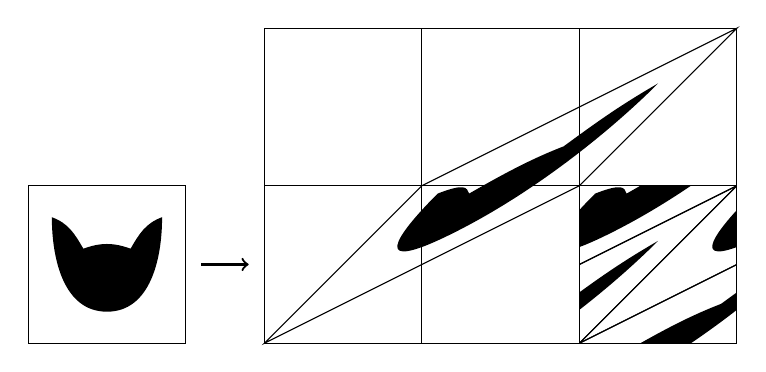
\begin{tikzpicture}[deforme/.style={ yslant=0.5, xslant=2, yscale=0.5, xscale=2}]
    % non-deformed cat
    \Cat

    % grid 3x2
    \draw[xshift=3cm, step=2cm, thin] (0,0) grid (6,4);

    % arrow
    \draw[->, thick] (2.2, 1) -- (2.8,1);

    % deformed cat full
    \begin{scope}[xshift=3cm, deforme]
        \Cat
    \end{scope}

    % deformed cat cut
    \clip[draw] (7,0) rectangle ++(2,2);
    \begin{scope}[xshift=5cm, deforme]
        \Cat
    \end{scope}
    \begin{scope}[xshift=5cm, yshift=-2cm, deforme]
        \Cat
    \end{scope}
    \begin{scope}[xshift=3cm, yshift=-2cm, deforme]
        \Cat
    \end{scope}
    \begin{scope}[xshift=7cm, deforme]
        \Cat
    \end{scope}
\end{tikzpicture}
